% !TEX encoding = UTF-8 Unicode

\documentclass[a4paper]{article}

\usepackage{color}
\usepackage{url}
\usepackage[T2A]{fontenc} % enable Cyrillic fonts
\usepackage[utf8]{inputenc} % make weird characters work
\usepackage{graphicx}
\graphicspath{ {slike/} }

\usepackage[english,serbian]{babel}
%\usepackage[english,serbianc]{babel} %ukljuciti babel sa ovim opcijama, umesto gornjim, ukoliko se koristi cirilica

\usepackage[unicode]{hyperref}
\hypersetup{colorlinks,citecolor=green,filecolor=green,linkcolor=blue,urlcolor=blue}

%\newtheorem{primer}{Пример}[section] %ćirilični primer
\newtheorem{primer}{Primer}[section]

\begin{document}

\title{Asembliranje sekvenci\\ \small{Seminarski rad u okviru kursa\\Uvod u bioinformatiku\\ Matematički fakultet}}

\author{Aleksandra Karadžić, Dragutin Ilić\\ karadzic.matf@gmail.com, dragutin\_ilic@yahoo.com}
\date{18.~maj 2017.}
\maketitle

\abstract{
U ovom tekstu je ukratko prikazana osnovna forma seminarskog rada. Obratite pažnju da je pored ove .pdf datoteke, u prilogu i odgovarajuća .tex datoteka, kao i .bib datoteka korišćena za generisanje literature. Na prvoj strani seminarskog rada su naslov, apstrakt i sadržaj, i to sve mora da stane na prvu stranu! Kako bi Vaš seminarski zadovoljio standarde i očekivanja, koristite uputstva i materijale sa predavanja na temu pisanja seminarskih radova. Ovo je samo šablon koji se odnosi na fizički izgled seminarskog rada (šablon koji \emph{morate} da ispoštujete!) kao i par tehničkih pomoćnih uputstava. Molim Vas da kada budete predavali seminarski rad, imenujete datoteke tako da sadrže temu seminarskog rada, kao i imena i prezimena članova grupe (ili samo temu i prezimena, ukoliko je sa imenima predugačko). Predaja seminarskih radova biće isključivo preko web forme, a NE slanjem mejla.

\tableofcontents

\newpage

\section{Uvod}
\label{sec:uvod}

Sekvenciranje genoma, odnosno određivanje rasporeda nukleotida (nt) u genomu, je jedan od fundamentalnih zadataka u bioinformatici. Dužina genoma varira u zavisnosti od organizma (dužina ljudskog genoma je oko 3 milijarde nt, a jedan od najdužih genoma pripada amorfnom jednoćelijskom organizmu \textit{Ameoba dubia} koja je oko 200 puta duži). Najveća prepreka je zapravo činjenica da još uvek nisu razvijene tehnologije koje omogućavaju čitanje nukleotida u genomu od početka do kraja (slično kao čitanje stranica knjige sleva udesno). Trenutno zastupljeno rešenje je sekvenciranje manjih fragmenata DNK koji se nazivaju \textbf{ridovi (\textit{eng. reads})}. Uzima se mali uzorak tkiva ili krvi koji sadrži milione kopija DNK. Biohemijskim procesima se DNK razbija na fragmente, čijim sekvenciranje se dobijaju ridovi. Ne zna se iz kog dela genoma je dobijen određeni rid, pa se koristi tehnika preklapanja ridova da bi se rekontruisao genom. Ovaj ceo proces se naziva i \textbf{asembliranje genoma (\textit{eng. genome assembly})}. \\
\indent Prvo sekvenciranje genoma je odrađeno 1977. godine od strane Frederika Sangera (eng. Frederick Sanger). U Sangerovom metodu dužina ridova je bila između 500 i 1000 ridova. Većina programa zasnovana na ovoj tehnici (\textit{eng. de novo assembly programs}) se bazira na strategiji  "preklapanje-raspored-konsenzus" (\textit{eng. overlap-layout-consensus strategy}), u kojoj se preklapanja između ridova izračunavaju brzim tehinikama upore\-đivanja, raspored kontiga (\textit{eng. contigs}) se generiše pomoću preklapanja u opadajućem rasporedu kvaliteta, a konsenzus sekvenci kontiga se dobija brzim metodama višestrukog poravnavanja. Glavni razlog uspešnosti ovih programa jeste ta da je veličina ridova dovoljna za ustanovljavanje razlika između pravih i lažnih preklapanja. \\
\indent Prilikom sekvenciranja genoma nailazimo na otežavajuće situacije.Prvo, DNK se sastoji od dve niti, pa ne možemo znati iz koje od njih je rid izveden (nemamo inforamciju da li da koristimo dobijen rid ili njegov obrnuti komplement prilikom asembliranja određene niti u genomu). Drugo, tehnologije koje se koriste nisu savršene, pa dobijeni ridovi često sadrže greške (čime se otežava preklapanje ridova). Treće, neki regioni genoma mogu da ostanu nepokriveni ridovima, čime je onemogućena rekonstrukcija celog genoma. Za otklanjanje ovih problema se koriste razne tehnike kao na primer: pristup razbijanja ridova (\textit{eng. read breaking 
approach}) se koristi za problem nepokrivenosti genoma ridovima, asembliranje kontiga (neprkidnih delova genoma), a ne čitavih hromozoma, se vrši zbog navedenih problema,tehnika uklanjanja mehurova (\textit{eng. bubble removal}) kojom se rešavaju ridovi sa greškom (lažni ridovi) itd. \\
\indent Sa ulaskom u drugu genereciju (masovno paralelnih) sekvencijalnih tehnologija, počelo se sa proizvodnjom na milijarde kratkih ridova dužine od 50 do 150 nukleotida. Ogromni skupovi podataka vremenski i prostorno usložnjavaju izra\-čuna\-va\-nje preklapanja dinamičkim algoritmima. Ridovi male dužine otežavaju otkrivanje tačnih od lažnih preklapanja prilikom generisanja rasporeda kontiga. Kako bi se ovo izbeglo, razvijeni su algoritmi za asembliranje zasnovani na detekciji preklapanja kao tačnih pogodataka fiksne dužine. Na osnovu ovakvih preklapanja formira se \textit{de Bruijin}-ov graf, u kome svaki jedinstevni string dužine k (k-mer) koji se pojavljuje u ridu, predstavlja granu koja spaja čvorove označene sa k-1-mer prefiksom i k-1-mer sufiksom. Pomoću ovog grafa i distribucije frekvencije stringova u ridovima razlikujemo stringove koji imaju grešku od onih koji nemaju. Stringovi sa greškama se ili ne koriste ili se prepravljaju i zatim koriste pri asembliranju.  \\
\indent Kako bi koristili sekvenciranje ridova direktno, u ovom radu je predstavljen efikasan metod za izračunjavanje preklapanja za kratke ridove. Metod dozvoljava promašaje u preklapanjima, ali ne dodavanja i brisanja, koji se inače i javljaju ređe od promašaja. U grafu preklapanja, svaki čvor predstavlja rid, dok grana predstavlja preklapanje. U ovom grafu algoritam pronalazi jedinstvenu putanju ridova koja reprezentuje kontigu. Konsenzus sekvence svake kontige je dobijen izračunavanjem poravnanja višestrukih ridova koji nisu razdvojeni nukleotidima koji oni ne sadrže. \\
\indent U nastavku će biti predstavljni detalji algoritma kao i opis programa PCAP.Solexa u kome je algoritam implementiran.
\iffalse
\begin{primer}
Problem zaustavljanja (eng.~{\em halting problem}) je neodlučiv \cite{haltingproblem}.
\end{primer}

\begin{primer}
Za prevođenje programa napisanih u programskom jeziku C može se koristiti GCC kompajler \cite{gcc}.
\end{primer}

\begin{primer}
 Da bi se ispitivala ispravost softvera, najpre je potrebno precizno definisati njegovo ponašanje \cite{laski2009software}. 
\end{primer}
Reference koje se koriste u ovom tekstu zadate su u datoteci {\em seminarski.bib}. Prevođenje u pdf format u Linux okruženju može se uraditi na sledeći način:

\begin{verbatim}
pdflatex TemaImePrezime.tex 
bibtex TemaImePrezime.aux 
pdflatex TemaImePrezime.tex 
pdflatex TemaImePrezime.tex 
\end{verbatim}
Prvo latexovanje je neophodno da bi se generisao {\em .aux} fajl. {\em bibtex} proizvodi odgovarajući {\em .bbl} fajl koji se koristi za generisanje literature. 
Potrebna su dva prolaza (dva puta pdflatex) da bi se reference ubacile u tekst (tj da ne bi ostali znakovi pitanja umesto referenci). Dodavanjem novih referenci potrebno je ponoviti ceo postupak.  


Broj naslova i podnaslova je proizvoljan. Neophodni su samo Uvod i Zaključak. Na poglavlja unutar teksta referisati se po potrebi. 
\begin{primer}
U odeljku \ref{sec:naslov1} precizirani su osnovni pojmovi, dok su zaključci dati u odeljku \ref{sec:zakljucak}.
\end{primer}

\fi



\section{Opis algoritma}
\label{opis_algoritma}
Na početku ćemo opisati metod koji se koristi za izračunavanje preklapanja izmedju ridova. Za realizaciju ovog metoda je korišćena struktura podataka koju ćemo zvati \textbf{``niz super-reč''} (\textit{eng. superword array}), koja je ime dobila na sličan način kao i druga struktura podataka zvana ``sufiksni niz'' (\textit{eng. sufix array}). Reč dužine \textit{w} je string od \textit{w} karaktera, a super-reč sa \textit{v} reči je string sa \textit{v*w} karaktera dobijena konkatenacijom tih reču po redu u kome se javljaju. Reči u super-reči ćemo indeksirati pozicijama od 1 do \textit{v}. Pozicije u rečima (indeksiranje kreće od jedinice) se dele u dve grupe: čekirane i nečekirane poicije. Za dve reči dužine \textit{w} kažemo da se podudaraju ukoliko imaju identične nukleotide na svakoj čekiranoj poziciji tih reči. Na primer ako imamo dve reči dužine 15, \textbf{ACCATACCATAGCAC} i \textbf{ACTATTCCATAACAC}, i ako pretpostavimo da su nečekirane pozicije 3,6 i 12 tada za ove dve reči možemo reći da se podudaraju. Dužina reči \textit{w} se često namešta da bude 12 ili veća, kako bi broj čekiranih pozicija u reči bio 12, čime se osigurava da lookup tabela za sve stringove ove dužine (ako je reč duža od 12 brišemo sve nukleotide iz nečekiranih pozicija) može stati u glavnu memoriju. Broj reči \textit{v} se bira tako da super-reč dužine \textit{v*w} bude manja od dužine svakog rida (dužinu rida ćemo označavati sa  \textit{r}). Dužina super-reči se još naziva i minimalna dužina preklapanja. Adekvatan primer za ridove dužine 150 bi bio da postavimo da \textit{w} na 15 i \textit{v} na 6 čime dobjamo super-reči dužine 90. Rid dužine \textit{r} ima \textit{r - w*v }+ 1 super-reči na pozicijama 1,2, \ldots ,\textit{r - w*v }+ 1. U našem primeru bi rid dužine 150 imao 61 super-reč na pozicijama 1,2, \ldots ,61. Za dve super-reči kažemo da su identične ako im se sve reči podudaraju, odnosno svi nukleotidi na čekiranim pozcijama su im identični. Za jednu super-reč kažemo da je manja (veća) od druge ako string nukleotida na svakoj čekiranoj poziciji prve super-reči, u lekiskografskom poredku, dolazi pre (posle) stringa nukleotida na čekiranim pozicijama druge super-reči. Svaki rid dobija jedinstveni nenegativni ceo broj koji se zove indeks rida. Pomoću njega i početne pozicije super-reči u ridu se izračunava jedinstveni indeks svake super-reči u svakom ridu. U algoritmu se koristi i funkcija koja pomoću datog indeksa super-reči efikasno računa poziciju te super-reči u indeksu i indeks rida.Sada imamo sve podatke kako bi definisali ``niz super-reč'' strukturu podataka. \textbf{``Niz super-reč''} za skup ridova je niz svih indeksa super-reči gde su super-reči sortirane od manje ka većoj.

\begin{figure}[h!]
\begin{center}
\end{center}
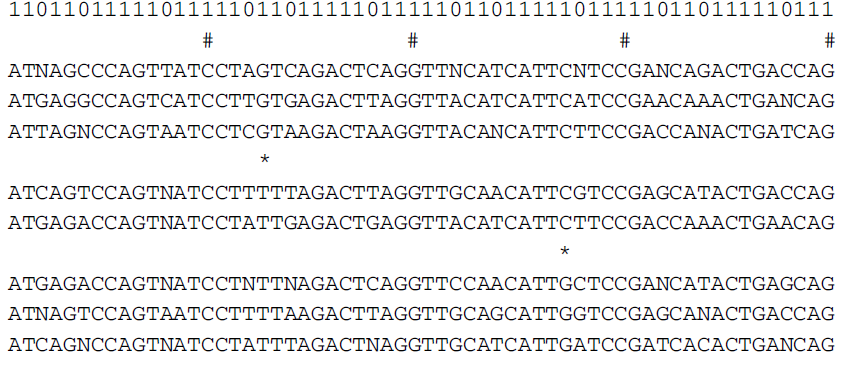
\includegraphics[width=\textwidth]{superreci}
\label{fig:superreci}
\caption{Prikaz grupisanja i sortiranja super-reči}
\end{figure}

\indent Na slici \ref{fig:superreci} prikazano je osam super-reči u sortiranom poredku. Svaka super-reč se sastoji od četiri reči (v=4) dužine w = 15, gde je svaka čekirana pozicija označena bitom 1 , a nečekirana 0. Poslednja pozicija svake reči je označena taraba znakom. Super-reči su grupisane tako da se u svakom bloku nalaze identične super-reči (prve tri, sledeće dve i poslednje tri). Vidimo da nukleotidi na nečekiranim pozicijama mogu biti ili različiti ili nedefinisani (označeni sa \textbf{N}) u istom bloku. Pvi blok dolazi pre drugog zato što na poziciji označenoj sa zvezdicom se u prvom bloku nalazi \textbf{G} nukleotid a u drugom \textbf{T} (\textbf{G} leksikografski dolazi pre \textbf{T}). Slično zvezdica izmedju drugog i trećeg bloka označava zašto drugi dolazi pre trećeg.
\subsection{Konstrukcija niza super-reč}
\label{subsec:knsr}
 Niz super-reč se konstriše pomoću bucket sorta u \textit{v} krugova sortiranja (podsetimo se da se svaka super-reč sastoji od \textit{v} reči od kojih svaka ima tačno 12 čekiranih pozicija). Najpre se niz inicializuje indeksima super-reči u rastućem poretku po vrednostima indeksa. Zatim se iz svake super-reči uzima reč na poziciji \textit{p} gde \textit{p} ide od \textit{v} do 1 (krećemo se sdesna u levo u svakoj super-reči) i niz sortiramo po leksikografskom poretku tih reči. Kako idemo sdesna u levo nakon \textit{v} koraka bucket sort garantuje da će ``niz super-reč'' biti sortiran. Za sortiranje se koriste dve pomocne strukture podataka, lookup tabela i niz lokacija , koji služe kao kofe (\textit{eng. bucket}) u koje smeštamo reči. Niz lokacija je niz celih brojeva koji je indeksiran od 0 do najvećeg indeksa super-reči. Lookup tabela se inicijalizuje negativnim brojevima što označava praznu kofu, a ima onoliko polja koliko ima kodova za sve stringove dužine 12. Bucket sortiranje se obavlja tako što se elementi ``niza super-reč'' sleva na desno  čitaju ,smeštaju u kofe i zatim se kopiraju iz kofa nazad u ``niz super-reč'' sdesna u levo. Detaljnije, trenutni element, indeks super-reč,i se smešta u kofu iz ``niza super-reč'' na sledeći način. Indeks super-reči se koristi kako bi se našla reč na poziciji \textit{p}. Zatim   tu reč koja je dužine \textit{w} transformišemo u string dužine 12 korišćenjem bitovskih operacija kako bi uklonili nukleotide na nečekiranim pozicijama. Znamo da postoji indeks u lookup tabeli koji predstavlja kod tog stringa dužine 12, pa vrednost lookup tabele na tom indeksu čuvamo u nizu lokacija na poziciji koja ima isti indeks kao i indeks super-reči, a u lookup tabelu upisujemo sam indeks super-reči. Kada smo sve elemente ``niza super-reč'' ubacili u kofe, čitamo ih počevši od najveće kofe i kopiramo ih u ``niz super-reč'' sdesna ulevo.
\subsection{Izračunavanje preklapanja koristeći niz super-reč}
\label{subsec:ipknsr}
\indent Nakon konstrukcije ``niza super-reč'' delimo ga u sekcije tako da se u svakoj sekciji nalaze identične super-reči. Ove sekcije se obradjuju kako bi se generisala preklapanja izmedju ridova. To radimo na sledeći način. Posmatraćemo trenutnu sekciju koja ima \textit{s} super-reči. Svaka dva rida koja imaju super-reč u ovoj sekciji mogu da se poklapaju. Tako da imamao \((s*(s-1))/2\) potencijalnih preklapanja u ovoj sekciji. Kako bi uprostili problem mi nećemo računati sva ova preklapanja, već ćemo računati njegov podskup (koji ćemo dobiti za linearno vreme), a ostala preklapanja će moći da budu zaključena iz ovog podskupa. Ovo se može uraditi , tako što sortiramo super-reči u sekciji po dužini njihovih prefiksa u ridu i selektovanjem susednih parova super-reči kako bi izračunali preklapanja. Ako super-reči pripadaju različitim ridovima (podsetimo se da ovo možemo proveriti koristeći funkciju koja od indeksa super-reči računa poziciju super-reči u ridu i indeks rida kome ta super-reč pripada) onda računamo preklapanje izmedju njih. Ukoliko je broj nukleotida koji se razlikuju u preklapanju ograničen odsecanjem, preklapanje čuvamo.
\subsection{Ubrzanje paralelizacijom}
\label{subsec:up}
Veliki skupovi ridova se dele u manje podskupove (obeleženih brojevima od 0 do \textit{j}-1). Svaki rid iz istog podskupa ima super-reč kod koje ostatak pri deljenju koda reči na poziciji \textit{p} (\textit{p} je izmedju 1 i \textit{v}) sa \textit{j} daje oznaku tog podskupa. Naglasimo da rid može pripadati u više podskupova. Ovi podskupovi se dodeljuju \textit{j} procesorima kako bi se  paralelno izračunala preklapanja. Svaki procesor računa preklapanja u podskupu konstruišući niz super-reč za svaki podskup. Ovim postupkom dobijamo različite fajlove preklapanja za svaki podskup. Ovi fajlovi se potom skeniraju kako bi se uklonila redudantna preklapanja. Na taj način dobijamo skup  fajlova neredudantnih preklapanja. 
\subsection{Konstrukcija grafa preklapanja}
\label{subsec:kgp}
Fajlovi preklapanja se čitaju redom jadan po jedan i svako preklapanje sa dobrim procentom preklapanja (broj nukleotida koji su se razlikovali u preklapanju je manji od granice) čuvamo u glavnoj memoriji. Graf preklapanja se konstruiše da čvorovi budu ridova, a grane izmedju čvorova su preklapanja izmedju dva rida koju povezuje ta grana. Graf se potom ispituje kako bi se našle dugačke putanje preklapanja neponavljajućih čvorova. Čvor je ponavljajući ako postoje dve dugačke putanje koje se završavaju u čvoru, ali nemaju ponavljanja izmedju njihovih prefiksnih putanja. Ovo se izvodi na principu dijekstrinog algoritma. Svaka dugačka putanja neponavljajućih čvorova se predstavlja kao kontiga ridova. Stvaranje rasporeda svake kontige se obavlja na jednom procesoru sa velikom količinom glavne memorije. Na kraju ovog koraka se dobijaju fajlovi koji predstavljaju raspored kontiga.
\subsection{Generisanje fajla konsenzus sekvenci kontiga i ocene kvaliteta}
\label{subsec:gfkskiok}
 Fajlovi rasporeda kontiga se paralelno procesiraju. Ridovi se rasporedjuju kako bi formirali višestruka poravnanja ridova. Ova poravnanja se koriste za generisanje konsenzus sekvenci za kontige. Za svaki fajl rasporeda kontiga se generiše fajl konsenzus sekvenci kontiga kao i fajl ocene kvaliteta baza konsenzus kontiga. Na osnovu ovih fajlova se generiše jedan fajl konsenzus sekvenci kontiga i jedan fajl ocene kvaliteta baze konsenzus kontiga.

\iffalse


\begin{table}[h!]
\begin{center}
\caption{Razlčita poravnanja u okviru iste tabele ne treba koristiti jer su nepregledna.}
\begin{tabular}{|c|l|r|} \hline
centralno poravnanje& levo poravnanje& desno poravnanje\\ \hline
a &b&c\\ \hline
d &e&f\\ \hline
\end{tabular}
\label{tab:tabela1}
\end{center}
\end{table}

\end{primer}

\fi



\section{Prvi naslov}
\label{sec:naslov1}


Ovde pišem tekst. 
Ovde pišem tekst. 
Ovde pišem tekst. 
Ovde pišem tekst. 
Ovde pišem tekst. 
Ovde pišem tekst. 
Ovde pišem tekst. 
Ovde pišem tekst. 


%\subsection{Prvi podnaslov}
%\label{subsec:podnaslov1}

Ovde pišem tekst. 
Ovde pišem tekst. 
Ovde pišem tekst. 
Ovde pišem tekst. 
Ovde pišem tekst. 
Ovde pišem tekst. 
Ovde pišem tekst. 



Ovde pišem tekst. 
Ovde pišem tekst. 
Ovde pišem tekst. 
Ovde pišem tekst. 
Ovde pišem tekst. 
Ovde pišem tekst. 

\section{Drugi naslov}
\label{sec:naslov2}

Ovde pišem tekst. 
Ovde pišem tekst. 
Ovde pišem tekst. 
Ovde pišem tekst. 



Ovde pišem tekst. 
Ovde pišem tekst. 
Ovde pišem tekst. 
Ovde pišem tekst. 
Ovde pišem tekst. 
Ovde pišem tekst. 

\section{n-ti naslov}
\label{sec:naslovN}

Ovde pišem tekst. 
Ovde pišem tekst. 
Ovde pišem tekst. 
Ovde pišem tekst. 
Ovde pišem tekst. 

\subsection{... podnaslov}
\label{subsec:podnaslovK}

Ovde pišem tekst. 
Ovde pišem tekst. 
Ovde pišem tekst. 
Ovde pišem tekst. 
Ovde pišem tekst. 

\subsection{... podnaslov}
\label{subsec:podnaslovM}

Ovde pišem tekst. 
Ovde pišem tekst. 
Ovde pišem tekst. 
Ovde pišem tekst. 
Ovde pišem tekst. 

\section{Poslednji naslov}
\label{sec:naslovM}

Ovde pišem tekst. 
Ovde pišem tekst. 
Ovde pišem tekst. 
Ovde pišem tekst. 
Ovde pišem tekst. 
Ovde pišem tekst. 
Ovde pišem tekst. 
Ovde pišem tekst. 
Ovde pišem tekst. 

\section{Zaključak}
\label{sec:zakljucak}

Ovde pišem zaključak. 
Ovde pišem zaključak. 
Ovde pišem zaključak. 
Ovde pišem zaključak. 
Ovde pišem zaključak. 
Ovde pišem zaključak. 
Ovde pišem zaključak. 
Ovde pišem zaključak. 
Ovde pišem zaključak. 
Ovde pišem zaključak. 
Ovde pišem zaključak. 
Ovde pišem zaključak. 


\addcontentsline{toc}{section}{Literatura}
\appendix
\bibliography{seminarski} 
\bibliographystyle{plain}

\appendix
\section{Dodatak}
Ovde pišem dodatne stvari, ukoliko za time ima potrebe.
Ovde pišem dodatne stvari, ukoliko za time ima potrebe.
Ovde pišem dodatne stvari, ukoliko za time ima potrebe.
Ovde pišem dodatne stvari, ukoliko za time ima potrebe.
Ovde pišem dodatne stvari, ukoliko za time ima potrebe.


\end{document}
